%%----------------------------------------------------------------------------------------
\clearpage
\pagestyle{fancy}
%%----------------------------------------------------------------------------------------
%%       PREFAZIONE
%%----------------------------------------------------------------------------------------
\part{Le caratteristiche della sollecitazione interna}
\setcounter{section}{0}
\section{Le definizioni di $N$, $T$ ed $M$}
%--------------------------------------------------------------------------------------------------------------------------------------------------------------
\renewcommand{\thefigure}{11~-~1}
\begin{figure}[ht]
\centering
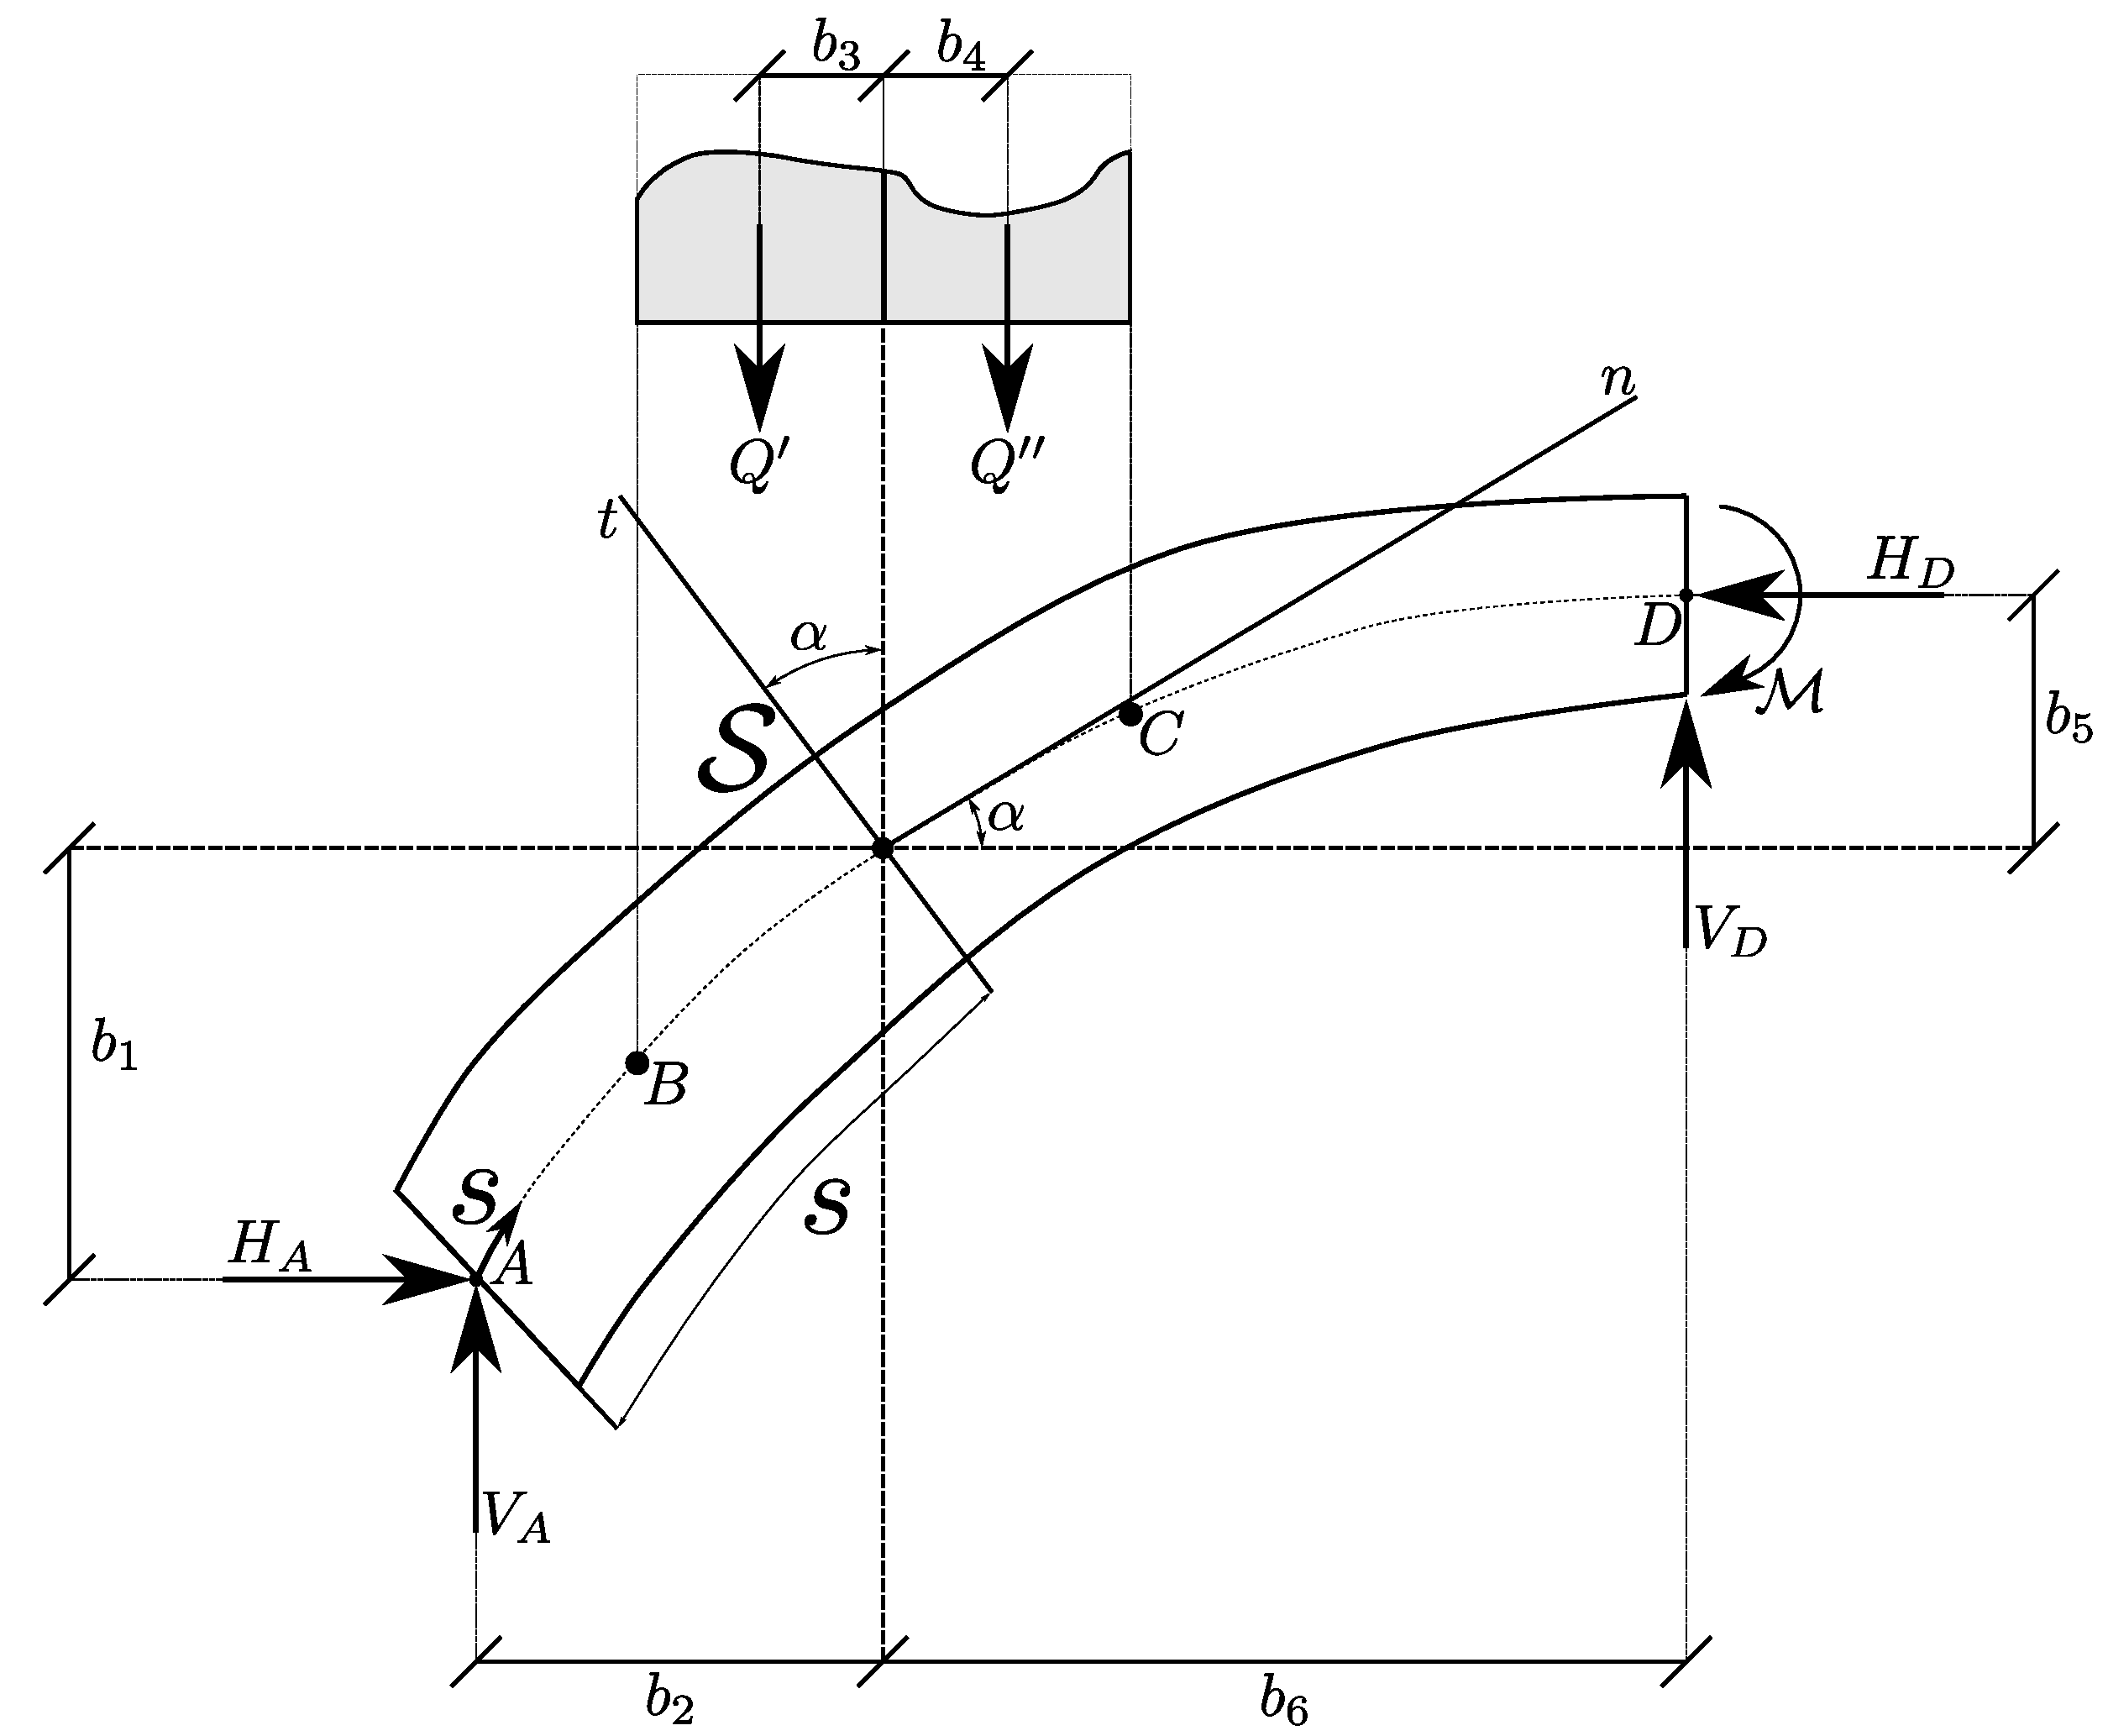
\includegraphics[width=0.89\textwidth]{Immagini/Parte_11/Figura11_1/figura11_1.pdf}
\caption{}
\label{figura11-1}
\end{figure}
%--------------------------------------------------------------------------------------------------------------------------------------------------------------
%----------------------------------------------------------------------------------------
\noindent In figura~\ref{figura11-1} è rappresentata una trave ad asse curvo; non importa la forma della sezione. Supponiamo che la trave sia in equilibrio sotto l'azione del carico $q$ distribuito sul tratto $BC$, delle forze $H_{A}$, $V_{A}$, $H_{D}$, $V_{D}$ e del momento $\mathcal{M}$; non importa se tali carichi siano attivi o reattivi. Assumiamo un sistema di ascisse curvilinee correnti lungo l'asse della trave, con origine in $A$; in tal modo, ogni punto dell'asse e, quindi, in ogni sezione della trave, è individuato dalla sua ascissa curvilinea $s$. La generica sezione $\mathcal{S}$ divide la trave in due parti: $A\mathcal{S}$, cioè la parte che precede $\mathcal{S}$, ed $\mathcal{S}D$, cioè la parte che segue. In corrispondenza della sezione $\mathcal{S}$ abbiamo segnato la retta normale al piano della sezione e, quindi, tangente all'asse, indicandola con $n$. Abbiamo anche segnato la retta $t$ perpendicolare ad $n$. Si indica poi con $\alpha$ l'angolo che $n$ forma con l'orizzontale e quindi $t$ con la verticale. Ed ecco la definizione di \textsc{sforzo normale} $N$:
%--------------------------------------------------------------------------------------------------------------------------------------------------------------
\\

\fbox{\begin{minipage}{38em}
\centering
\textsc{Si dice \textbf{sforzo normale} in $\mathcal{S}$ e si indica con $N$ la somma algebrica delle componenti secondo $n$ di tutte le forze che precedono o seguono $\mathcal{S}$. Nella suddetta somma algebrica si assumono \textbf{positivi} i contributi di \textbf{trazione}, cioè tendenti a staccare le parti $A\mathcal{S}$ ed $\mathcal{S}D$, e \textbf{negativi} quelli di \textbf{compressione}.}
\end{minipage}}\\
%--------------------------------------------------------------------------------------------------------------------------------------------------------------
%--------------------------------------------------------------------------------------------------------------------------------------------------------------
\renewcommand{\thefigure}{11~-~2}
\begin{figure}[ht]
\centering
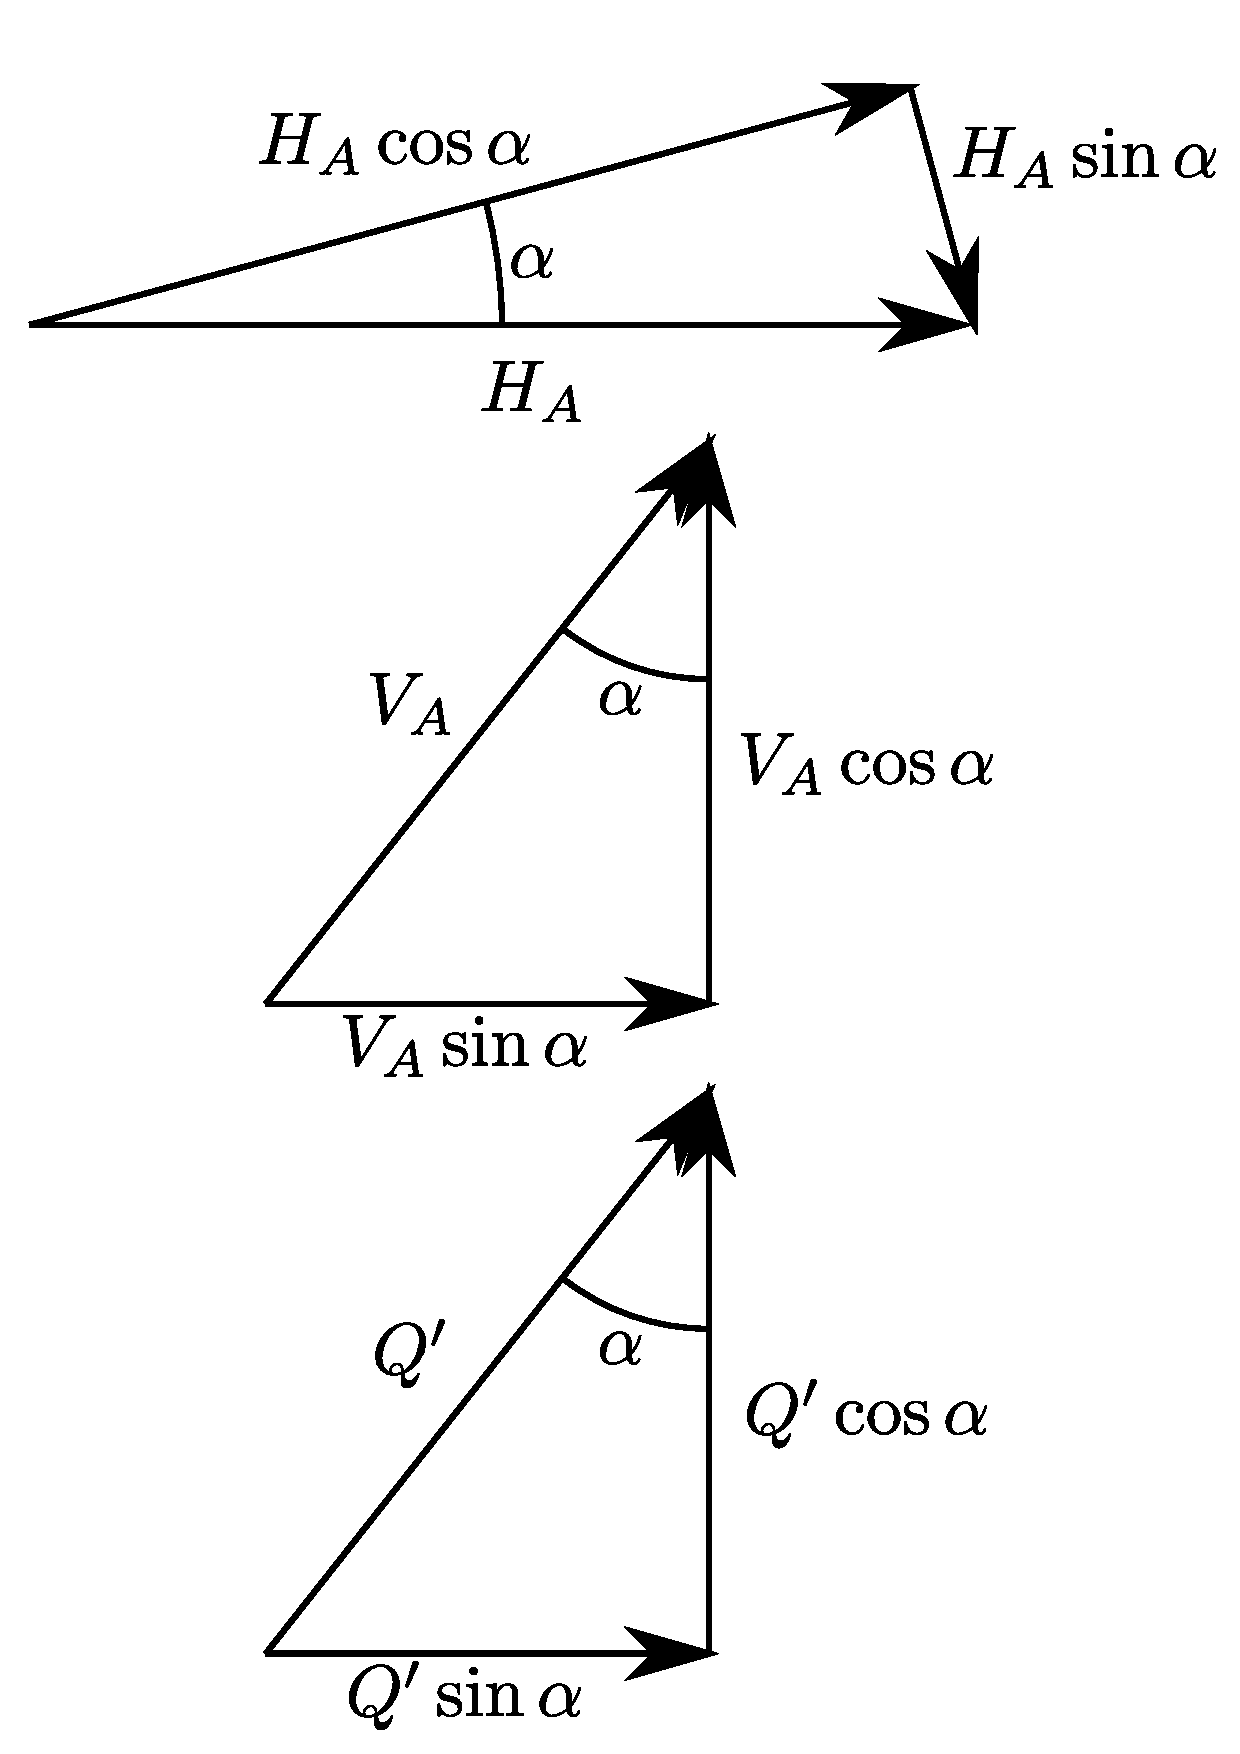
\includegraphics[width=0.4\textwidth]{Immagini/Parte_11/Figura11_2/figura11_2.pdf}
\caption{}
\label{figura11-2}
\end{figure}
%--------------------------------------------------------------------------------------------------------------------------------------------------------------

\noindent Calcoliamo, a titolo di esempio, lo sforzo normale nella sezione $\mathcal{S}$ in figura~\ref{figura11-2}, considerando le forze che precedono:
%--------------------------------------------------------------------------------------------------------------------------------------------------------------
\begin{equation} \label{equazione11-1}
\boxed{ N = - H_{A} \cos{\alpha} - V_{A}\sin{\alpha} + Q'\sin{\alpha} } \tag{11.1}
\end{equation}
%----------------------------------------------------------------------------------------
%--------------------------------------------------------------------------------------------------------------------------------------------------------------
\renewcommand{\thefigure}{11~-~3}
\begin{figure}[ht]
\centering
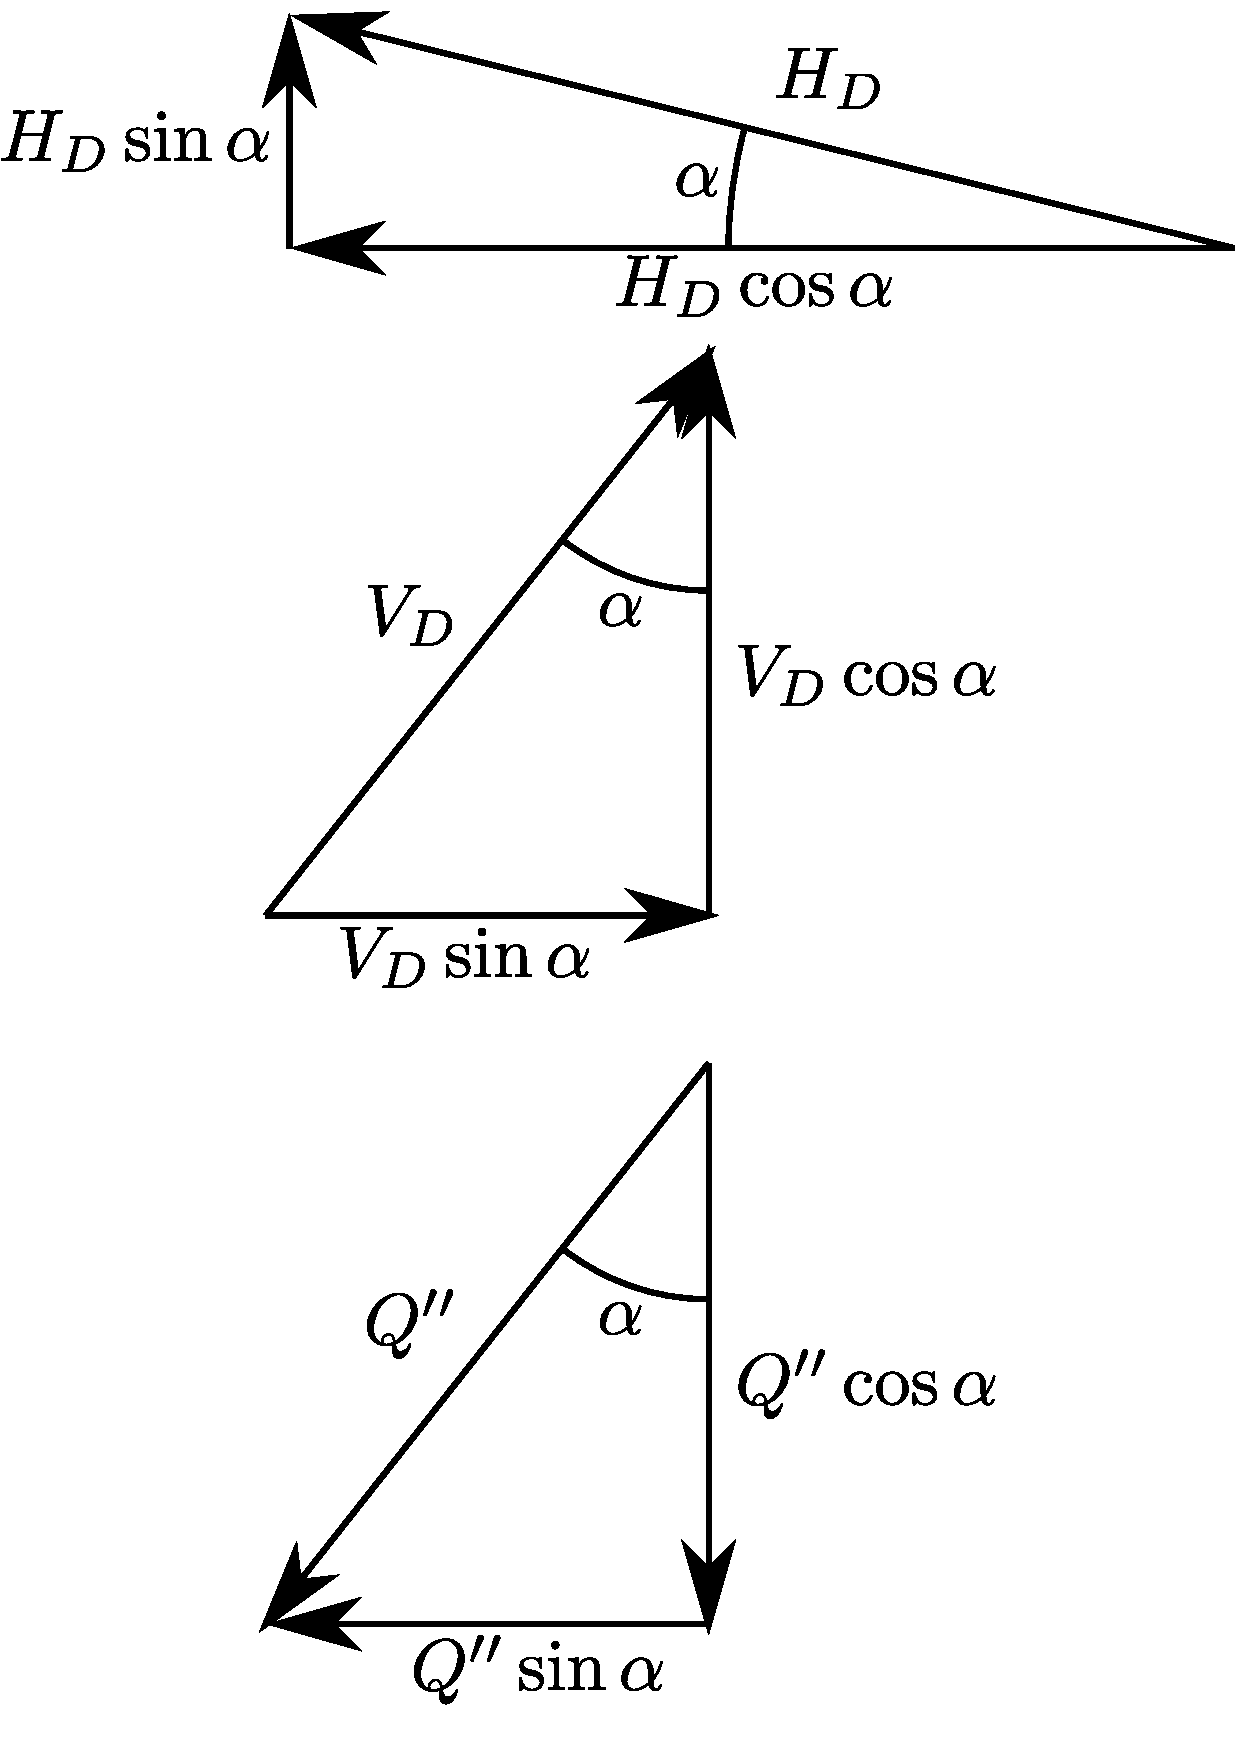
\includegraphics[width=0.4\textwidth]{Immagini/Parte_11/Figura11_3/figura11_3.pdf}
\caption{}
\label{figura11-3}
\end{figure}
%--------------------------------------------------------------------------------------------------------------------------------------------------------------
Considerando le forze che seguono come in figura~\ref{figura11-3}:
%----------------------------------------------------------------------------------------
\begin{equation} \label{equazione11-2}
\boxed{ N = - H_{D} \cos{\alpha} + V_{D}\sin{\alpha} - Q''\sin{\alpha} } \tag{11.2}
\end{equation}
%----------------------------------------------------------------------------------------
Le due espressioni di $N$ precedentemente trovate sono, ovviamente, uguali; per rendercene conto, basterà scrivere l'equazione di equilibrio alla traslazione lungo $n$ dell'intera trave; tenendo conto della figura, abbiamo
%----------------------------------------------------------------------------------------
\begin{equation*} 
H_{A} \cos{\alpha} + V_{A}\sin{\alpha} - Q'\sin{\alpha} - Q''\sin{\alpha} - H_{D} \cos{\alpha} + V_{D}\sin{\alpha}  = 0  
\end{equation*}
%----------------------------------------------------------------------------------------
e da questa relazione appena scritta
%----------------------------------------------------------------------------------------
\begin{equation} \label{equazione11-3}
\boxed{ -H_{A} \cos{\alpha} - V_{A}\sin{\alpha} + Q'\sin{\alpha} = -Q''\sin{\alpha} - H_{D} \cos{\alpha} + V_{D}\sin{\alpha} } \tag{11.3}
\end{equation}
%----------------------------------------------------------------------------------------
Dalla stessa definizione segue, ovviamente, che $N$ è funzione di $s$. Sempre con riferimento alla figura, ecco la definizione del \textsc{taglio}:
%--------------------------------------------------------------------------------------------------------------------------------------------------------------
\\

\fbox{\begin{minipage}{38em}
\centering
\textsc{Si dice \textbf{taglio} in $\mathcal{S}$ e si indica con $T$ la somma algebrica delle componenti secondo $t$ di tutte le forze che precedono o seguono $\mathcal{S}$. Nella suddetta somma algebrica si assumono \textbf{positivi} i contributi che risultano \textbf{antiorari} rispetto al baricentro della sezione $\mathcal{S}$.}
\end{minipage}}\\
%--------------------------------------------------------------------------------------------------------------------------------------------------------------

\noindent Calcoliamo, a titolo di esempio, il taglio nella sezione $\mathcal{S}$ mostrata in figura. Consideriamo le forze che precedono:
%----------------------------------------------------------------------------------------
\begin{equation} \label{equazione11-4}
\boxed{ T = H_{A}\sin{\alpha} - V_{A}\cos{\alpha} + Q'\cos{\alpha} } \tag{11.4}
\end{equation}
%----------------------------------------------------------------------------------------
Considerando, invece, le forze che seguono:
%----------------------------------------------------------------------------------------
\begin{equation} \label{equazione11-5}
\boxed{ T = -Q''\cos{\alpha} + H_{D}\sin{\alpha} + V_{D}\cos{\alpha} } \tag{11.5}
\end{equation}
%----------------------------------------------------------------------------------------
Per verificare l'uguaglianza delle espressioni di $T$ precedentemente trovate, basta scrivere l'equazione di equilibrio alla traslazione lungo $t$ dell'intera trave. Dalla stessa definizione segue, ovviamente, che $T$ è funzione di $s$. Ed ecco, infine, sempre con riferimento alla figura, la definizione di \textsc{momento flettente} $M$:
%--------------------------------------------------------------------------------------------------------------------------------------------------------------
\\

\fbox{\begin{minipage}{38em}
\centering
\textsc{Si dice \textbf{momento flettente} in $\mathcal{S}$ e si indica con $M$ la somma algebrica dei momenti rispetto all'asse perpendicolare al foglio e passante per il baricentro di $\mathcal{S}$ di tutte le forze e le coppie che precedono o seguono $\mathcal{S}$. Nella suddetta somma algebrica si assumono \textbf{positivi} i contributi \textbf{orari} se stiamo considerando le forze che \textbf{precedono}, \textbf{antiorario} se stiamo considerando le forze che \textbf{seguono}.}
\end{minipage}}\\
%--------------------------------------------------------------------------------------------------------------------------------------------------------------

\noindent Calcoliamo, a titolo di esempio, il momento nella solita sezione $\mathcal{S}$ della figura, andando a considerare le forze che precedono:
%----------------------------------------------------------------------------------------
\begin{equation} \label{equazione11-6}
\boxed{ M = -H_{A}\cdot b_{1} + V_{A}\cdot b_{2} - Q'\cdot b_{3} } \tag{11.6}
\end{equation}
%----------------------------------------------------------------------------------------
Considerando le forze che seguono: 
%----------------------------------------------------------------------------------------
\begin{equation} \label{equazione11-7}
\boxed{ M = H_{D}\cdot b_{5} + V_{D}\cdot b_{6} - Q''\cdot b_{4} } \tag{11.7}
\end{equation}
%----------------------------------------------------------------------------------------
Per verificare l'uguaglianza delle espressioni di $M$ precedentemente trovate, basta scrivere l'equazione di equilibrio alla rotazione dell'intera trave assumendo come polo il baricentro della sezione $\mathcal{S}$. Anche $M$, come $N$ e $T$, è chiaramente funzione di $s$. 
%--------------------------------------------------------------------------------------------------------------------------------------------------------------
%--------------------------------------------------------------------------------------------------------------------------------------------------------------
\clearpage
\section{Esercizi}
\paragraph{Esercizio 11.1}
%--------------------------------------------------------------------------------------------------------------------------------------------------------------
\renewcommand{\thefigure}{11.1~-~1}
\begin{figure}[ht]
\centering
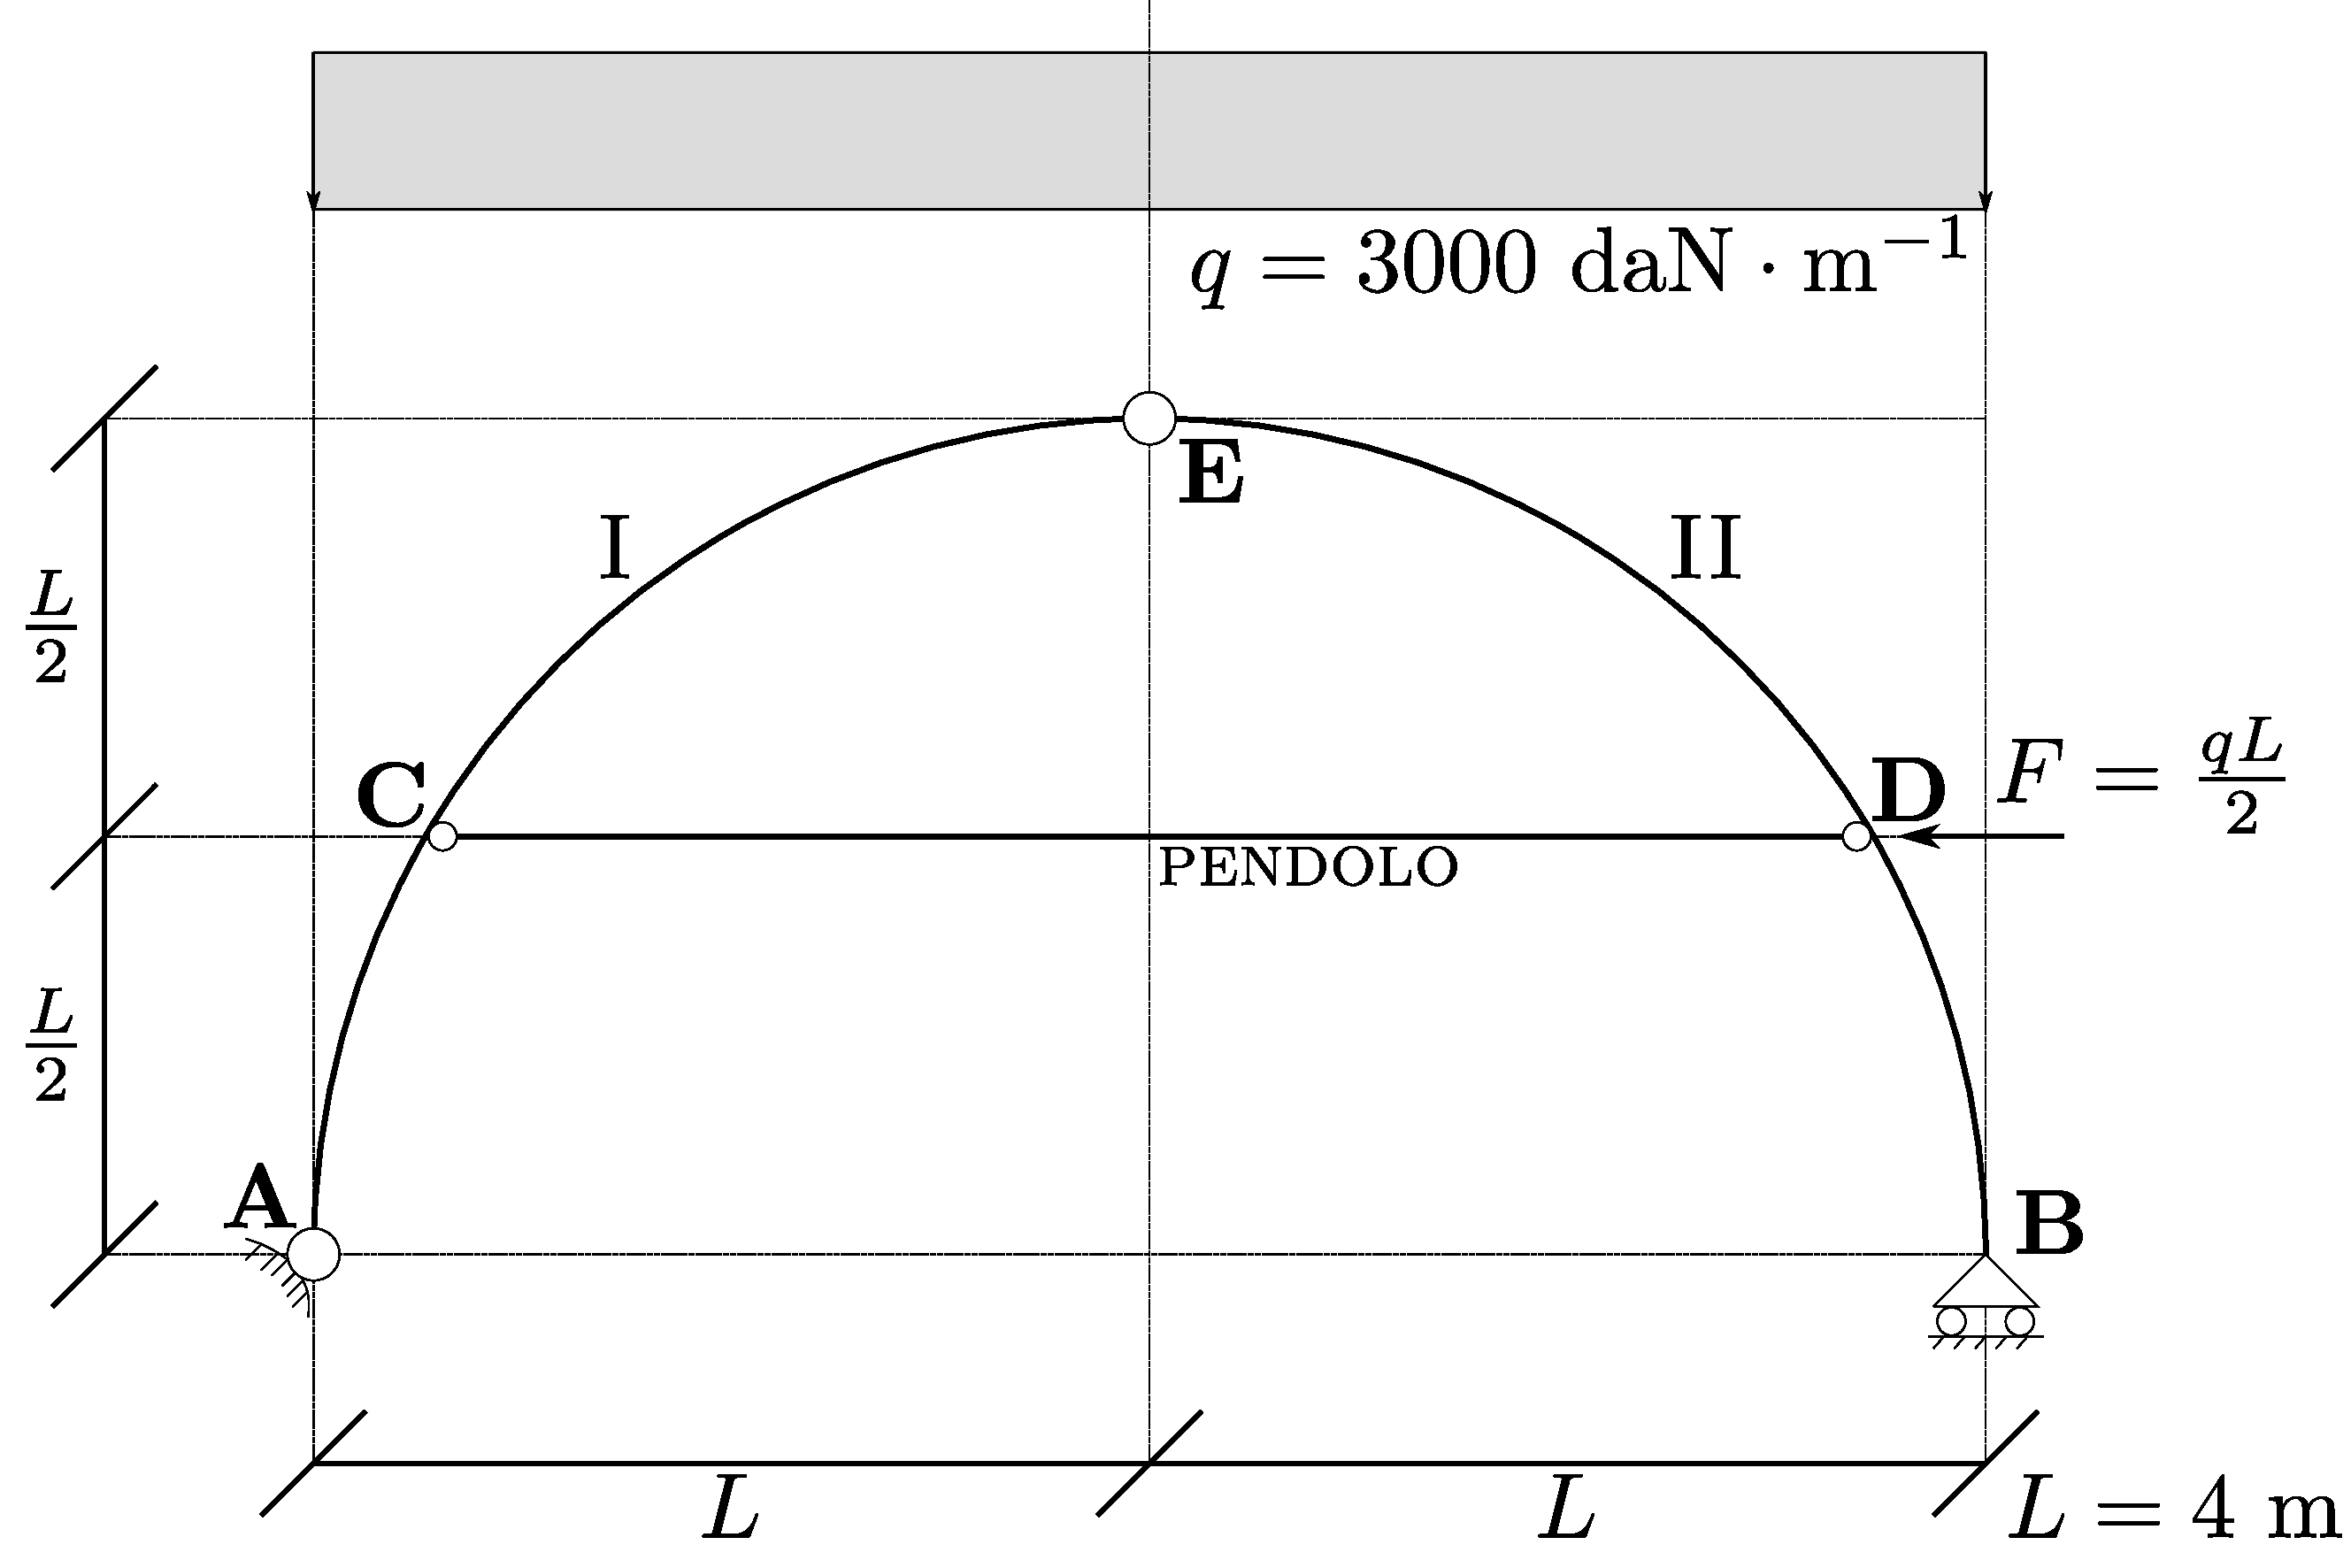
\includegraphics[width=0.75\textwidth]{Immagini/Parte_11/Esercizio11_1_1/esercizio11_1_1.pdf}
\caption{}
\label{Esercizio11-1-1}
\end{figure}
%--------------------------------------------------------------------------------------------------------------------------------------------------------------
%----------------------------------------------------------------------------------------
In figura~\ref{Esercizio11-1-1} è rappresentata la struttura da studiare; si tratta di una \textsc{semi}~-~\textsc{circonferenza}. Si chiede 
%----------------------------------------------------------------------------------------
\begin{enumerate}
\item di classificare la struttura;
\item di calcolare le reazioni vincolari; 
\item di calcolare $M$, $N$, e $T$ nelle sezioni $A$, $C_s$, $C_d$, $E_s$, $E_d$, $D_s$, $D_d$ e $B$. 
\end{enumerate}
%----------------------------------------------------------------------------------------
Si noti che con $C_s$ (si legga $C$ \emph{a sinistra}) si intende la sezione immediatamente prima di $C$ (spostandosi nel verso delle ascisse curvilinee) e con $C_d$ (si legga $C$ \emph{a destra}) quella immediatamente dopo; analogamente, questo discorso vale per i punti $E$ e $D$. 
%----------------------------------------------------------------------------------------
\subparagraph{Quesito 1}
%----------------------------------------------------------------------------------------
\begin{align*}
m &= 2\times 3 = 6 \\ 
n  &= 2A + 1B + 1p + 2E = 6 \\
\end{align*}
%----------------------------------------------------------------------------------------
Dunque
%----------------------------------------------------------------------------------------
\begin{equation*}
m - n = l - i = 0
\end{equation*}
%----------------------------------------------------------------------------------------
La cerniera in $E$ ed il pendolo rendono i due tronchi solidali; la cerniera in $A$ ed il carrello in $B$ impediscono al blocco rigido ogni movimento. Dunque, $l=i=0$ e la struttura è \textsc{isostatica}.
%----------------------------------------------------------------------------------------
\subparagraph{Quesito 2}
%----------------------------------------------------------------------------------------
Essendo la struttura isostatica per vincoli esterni, andiamo ad imporre l'equilibrio esterno: 
%----------------------------------------------------------------------------------------
\renewcommand{\thefigure}{11.1~-~2}
\begin{figure}[ht]
\centering
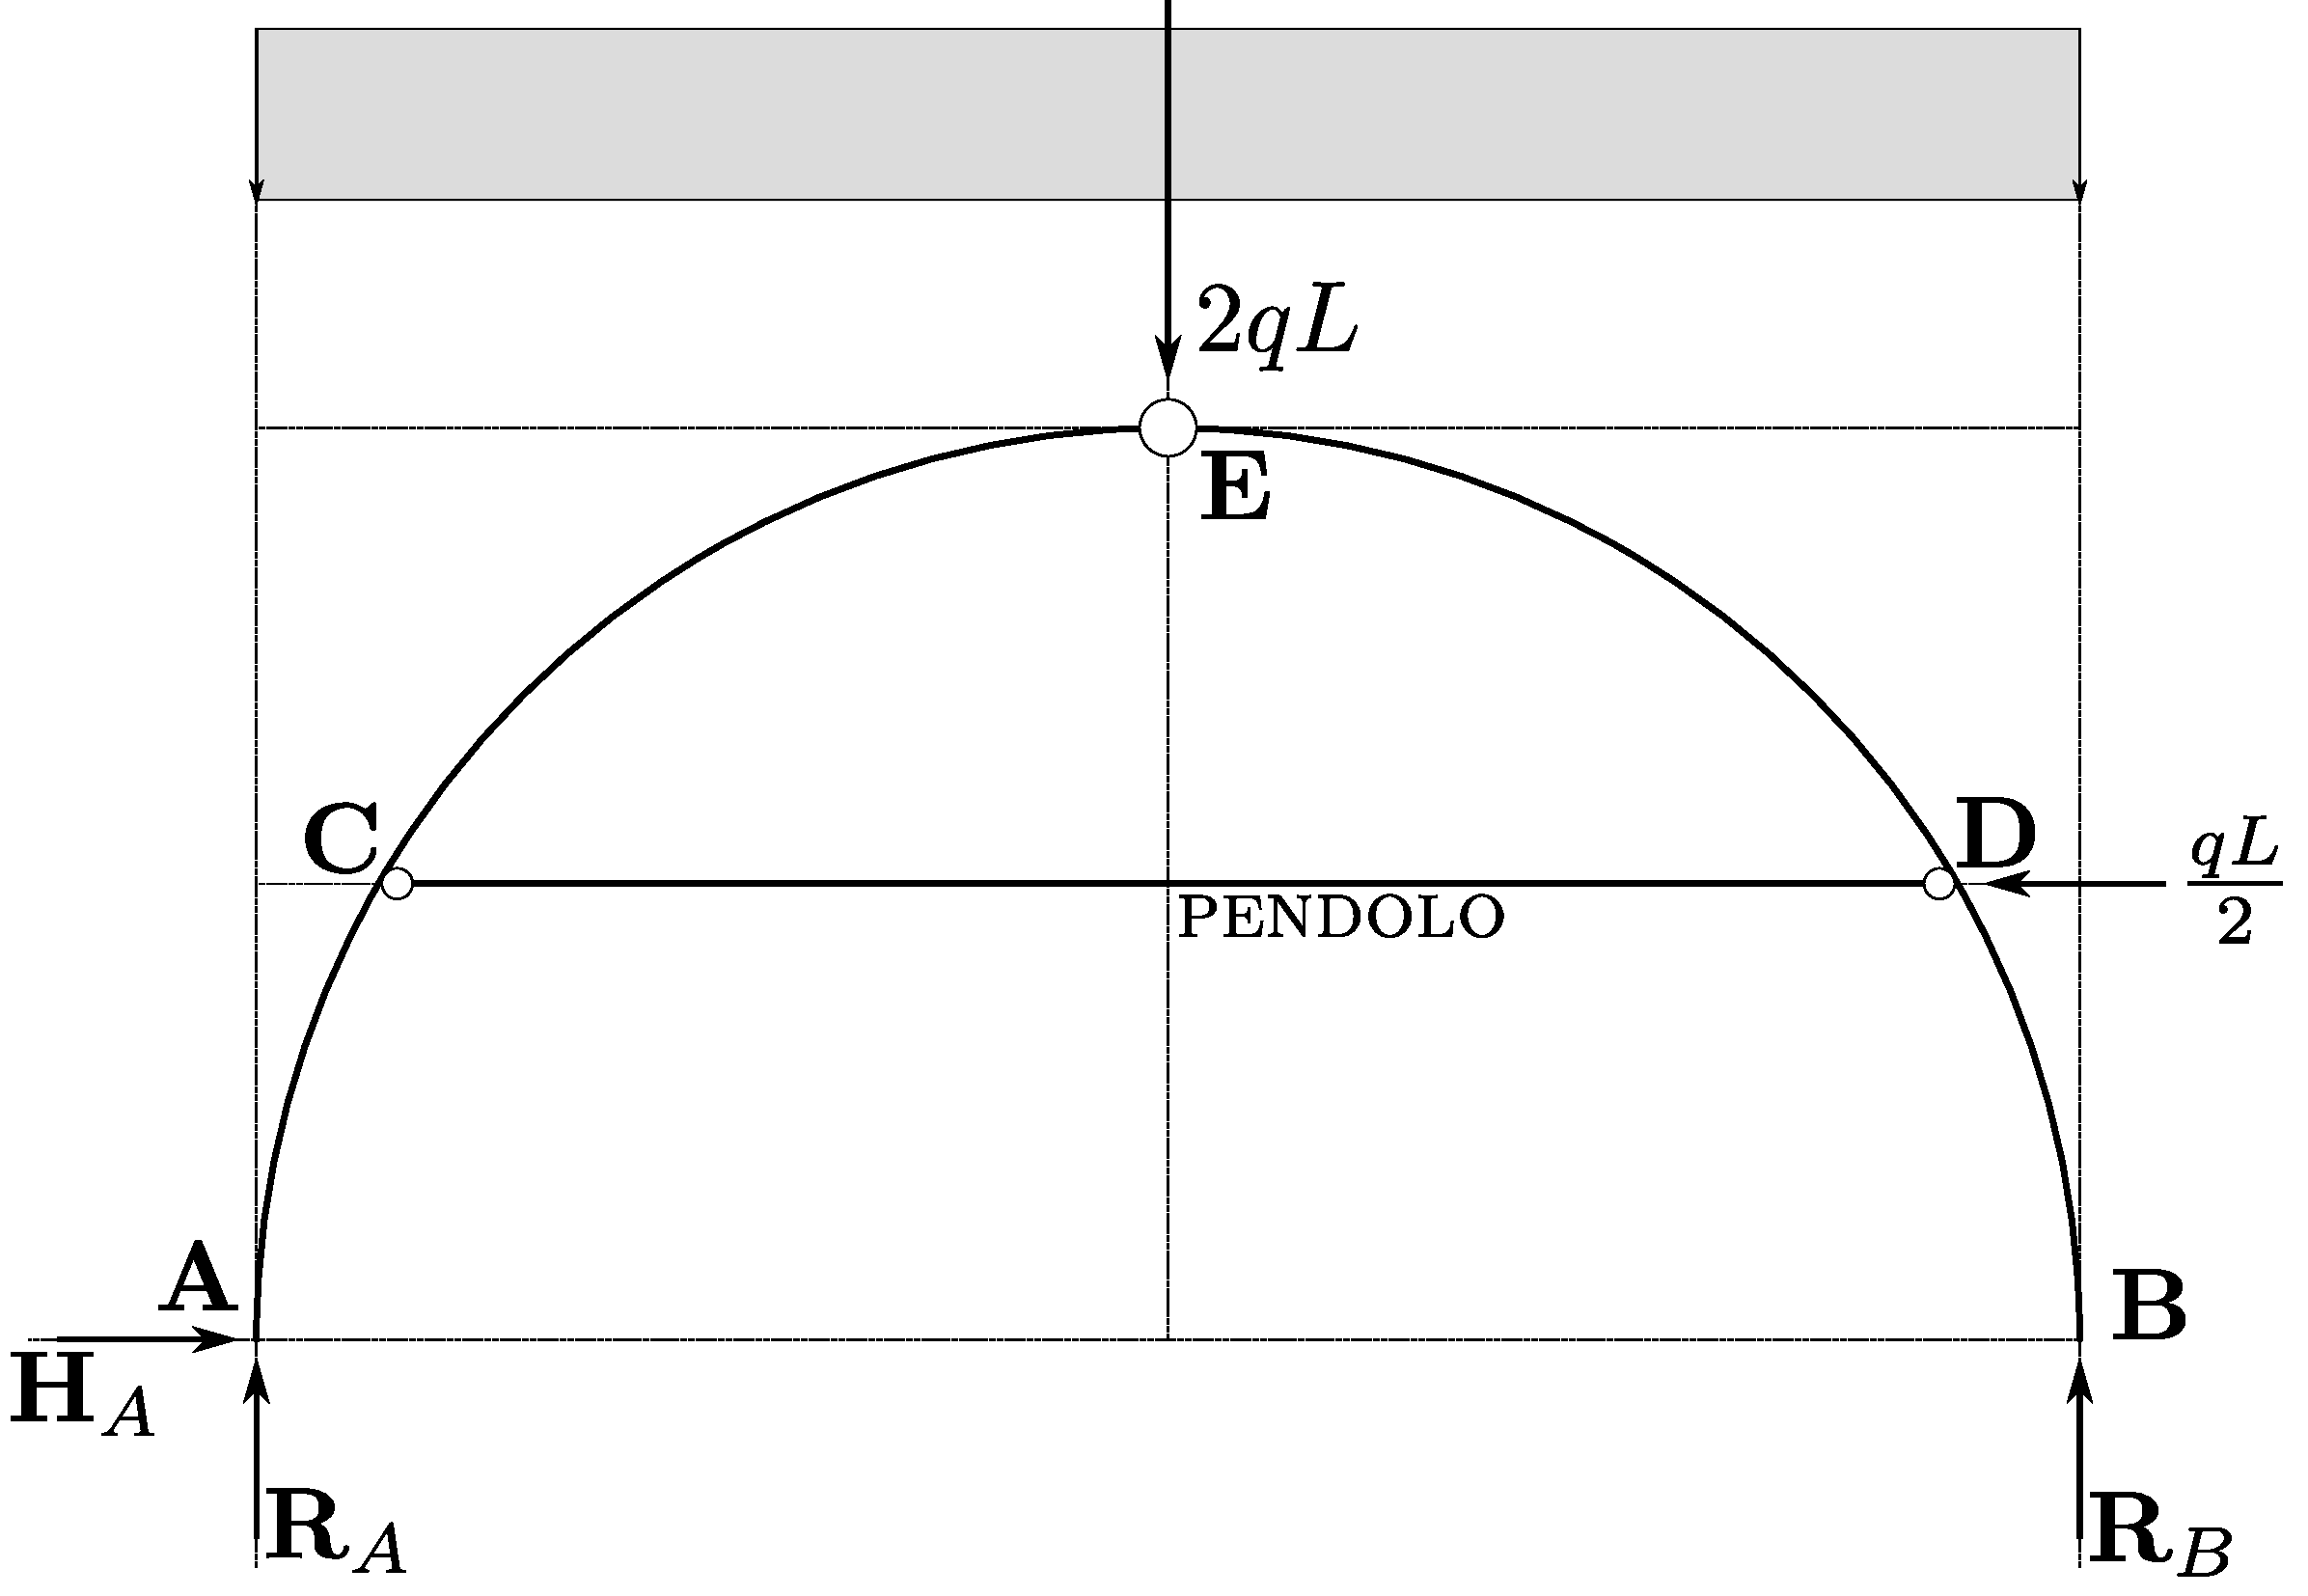
\includegraphics[width=0.75\textwidth]{Immagini/Parte_11/Esercizio11_1_1/esercizio11_1_2.pdf}
\caption{}
\label{Esercizio11-1-2}
\end{figure}
%----------------------------------------------------------------------------------------
Si osservi che, solo ai fini della scrittura delle equazioni di equilibrio esterno, è lecito sostituire il carico distribuito $q$ con la sua risultante. 
%----------------------------------------------------------------------------------------
\begin{subequations}
\begin{align}
H_{A} - \frac{qL}{2} &= 0 \quad [\rightarrow] \label{equazione11-1-1a} \tag{11.1.1a} \\
V_{A} + R_{B} - 2qL &= 0 \quad [\uparrow] \label{equazione11-1-1b} \tag{11.1.1b} \\ 
R_{B}\cdot 2L + \frac{qL}{2} \cdot \frac{L}{2} -2qL\cdot L &= 0 \quad [A\, \circlearrowleft] \label{equazione11-1-1c} \tag{11.1.1c}
\end{align}
\end{subequations}
%----------------------------------------------------------------------------------------
Abbiamo allora
%----------------------------------------------------------------------------------------
\begin{subequations}
\begin{align}
H_{A} &= \frac{qL}{2} \quad [\rightarrow] \label{equazione11-1-2a} \tag{11.1.2a} \\
R_{B} &= \frac{7}{8}qL \quad [\uparrow] \label{equazione11-1-2b} \tag{11.1.2b} \\ 
V_{A} &= \frac{9}{8}qL \quad [\uparrow] \label{equazione11-1-2c} \tag{11.1.2c}
\end{align}
\end{subequations}
%----------------------------------------------------------------------------------------
A questo punto entrambe i tronchi sono staticamente determinati; imponiamo l'equilibrio del primo tronco:
%----------------------------------------------------------------------------------------
\renewcommand{\thefigure}{11.1~-~3}
\begin{figure}[ht]
\centering
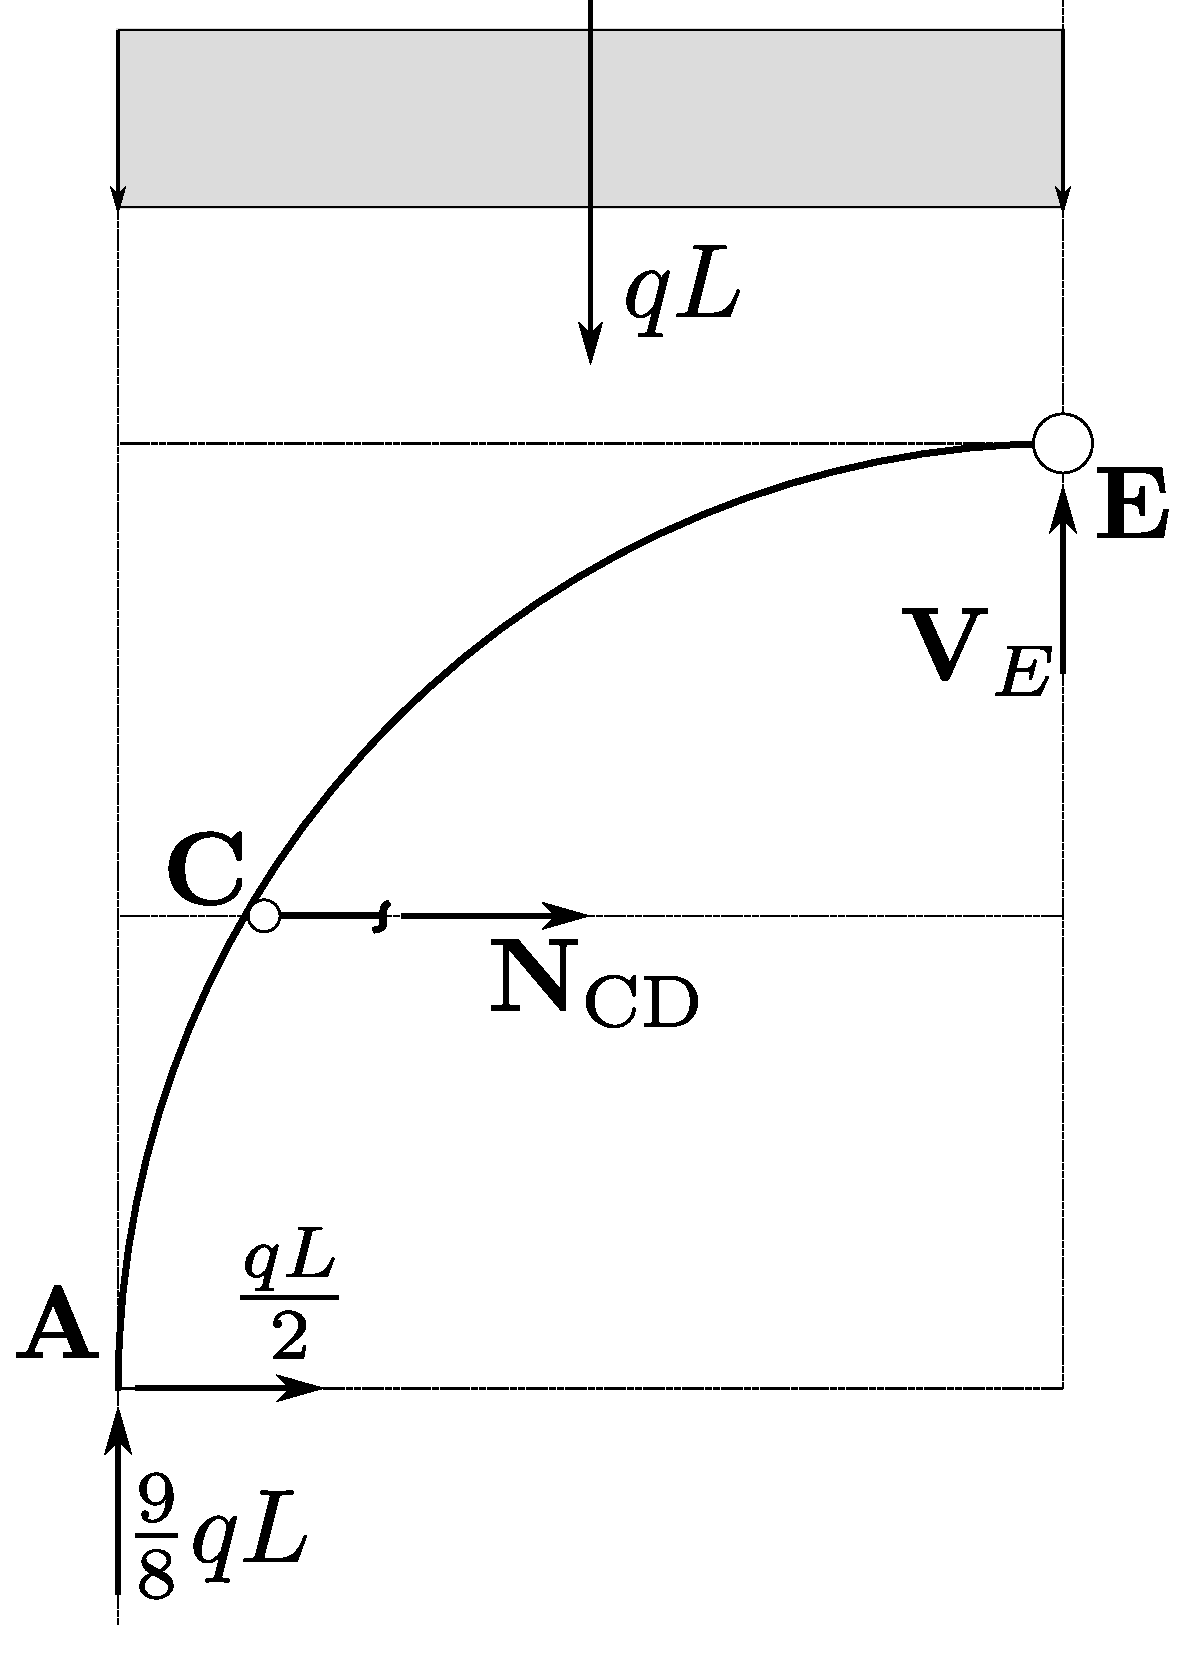
\includegraphics[width=0.45\textwidth]{Immagini/Parte_11/Esercizio11_1_1/esercizio11_1_3.pdf}
\caption{}
\label{Esercizio11-1-3}
\end{figure}
%----------------------------------------------------------------------------------------
Naturalmente, in figura~\ref{Esercizio10-1-3} è riportata la risultante della sola parte di carico che compete al primo tronco.
%----------------------------------------------------------------------------------------
\begin{subequations}
\begin{align}
\frac{qL}{2} + N_{\textup{CD}} + H_{E} &= 0 \quad [\rightarrow] \label{equazione11-1-3a} \tag{11.1.3a} \\
\frac{9}{8}qL - qL + V_{E} &= 0                  \quad [\uparrow] \label{equazione11-1-3b} \tag{11.1.3b} \\ 
-\frac{9}{8}qL\cdot L + \frac{qL}{2}\cdot L + N_{\textup{CD}} \cdot \frac{L}{2} + qL\cdot \frac{L}{2} &=0 \quad [E\, \circlearrowleft] \label{equazione11-1-3c} \tag{11.1.3c}
\end{align}
\end{subequations}
%----------------------------------------------------------------------------------------
Si ottiene 
%----------------------------------------------------------------------------------------
\begin{subequations}
\begin{align}
V_{E} &= - \frac{1}{8}qL \quad [\downarrow] \label{equazione11-1-4a} \tag{11.1.4a} \\
N_{\textup{CD}} &= \frac{qL}{4}                \quad [\text{Tirante}] \label{equazione11-1-4b} \tag{11.1.4b} \\ 
H_{E} &= - \frac{3}{4}qL \quad [\leftarrow] \label{equazione11-1-4c} \tag{11.1.4c}
\end{align}
\end{subequations}
%----------------------------------------------------------------------------------------
%----------------------------------------------------------------------------------------
\renewcommand{\thefigure}{11.1~-~4}
\begin{figure}[ht]
\centering
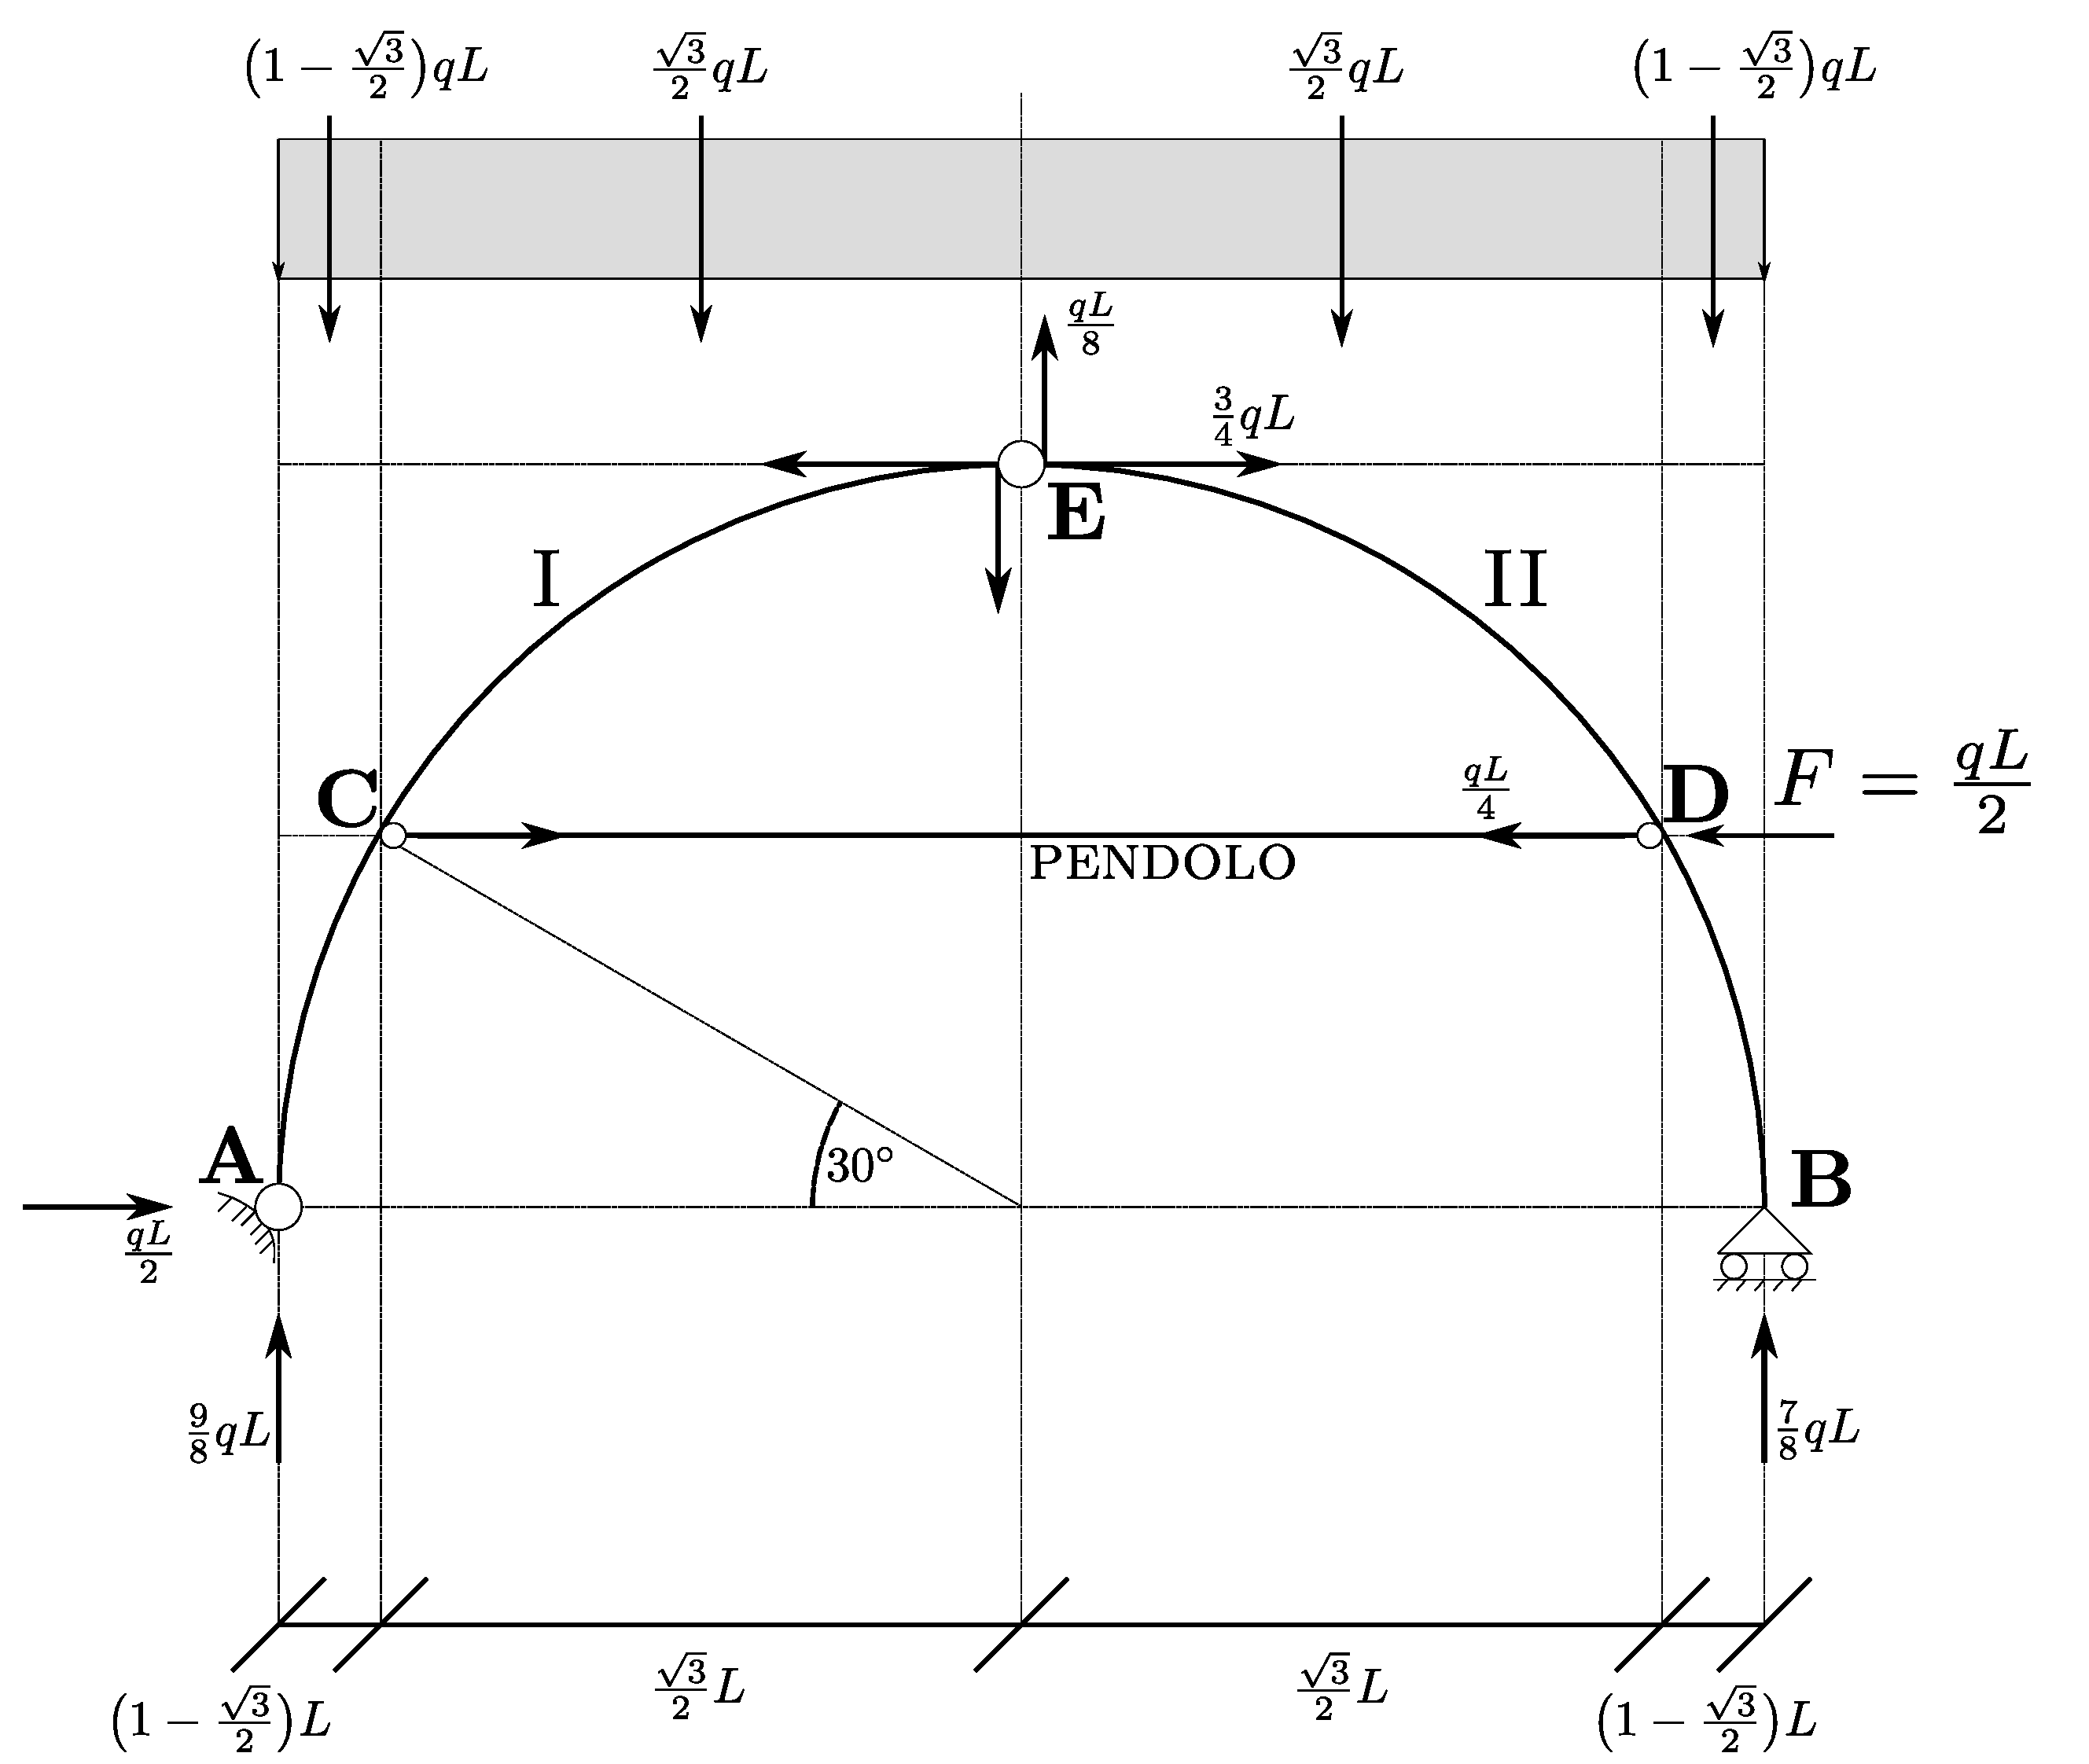
\includegraphics[width=\textwidth]{Immagini/Parte_11/Esercizio11_1_1/esercizio11_1_4.pdf}
\caption{}
\label{Esercizio11-1-4}
\end{figure}
%----------------------------------------------------------------------------------------
Ed ecco il quadro completo delle reazioni, rappresentato in figura~\ref{Esercizio11-1-4}. Al fine di calcolare le sollecitazioni nei punti $C$ e $D$, è stato necessario segnare le risultati delle forze che precedono e seguoni i suddetti punti; per tale motivo il carico distribuito è stato frazionato e sono riportate le relative risultanti parziali.
%----------------------------------------------------------------------------------------
\subparagraph{Quesito 3}
%----------------------------------------------------------------------------------------
\begin{equation*}
\text{Sezione A} 
\begin{cases}
M_{A} &= 0 \\
N_{A} &= - \frac{9}{8}qL = - \SI{13500}{daN} \\
T_{A} & = \frac{qL}{2}    = \SI{6000}{daN}
\end{cases}
\end{equation*}
%----------------------------------------------------------------------------------------
Per la sezione $C_s$ consideriamo le forze che precedono
%----------------------------------------------------------------------------------------
\begin{align*}
M_{\textup{C, s}} &= \frac{9}{8}qL \biggl( 1 - \frac{\sqrt{3}}{2} \biggr)\cdot L - \frac{qL}{2}\cdot \frac{L}{2} - \biggl( 1 - \frac{\sqrt{3}}{2} \biggr)\cdot qL \cdot \frac{1}{2} \cdot \biggl( 1 - \frac{\sqrt{3}}{2} \biggr) \cdot L = -\frac{\sqrt{3}}{16} qL^{2} = - \SI{5196}{daN.m} \\
N_{\textup{C, s}} &= -\frac{9}{8}qL \cdot \frac{\sqrt{3}}{2} - \frac{qL}{2}\cdot \frac{1}{2} + \biggl( 1 - \frac{\sqrt{3}}{2} \biggr) \cdot qL \cdot\frac{\sqrt{3}}{2} = - \frac{16+\sqrt{3}}{16} qL = - \SI{13299}{daN} \\
T_{\textup{C, s}} &=  -\frac{9}{8}qL \cdot \frac{1}{2} + \frac{qL}{2}\cdot \frac{\sqrt{3}}{2} + \biggl( 1 - \frac{\sqrt{3}}{2} \biggr)\cdot qL \cdot \frac{1}{2} = -\frac{1}{16}qL = -\SI{750}{daN}
\end{align*}
%----------------------------------------------------------------------------------------
per cui 
%----------------------------------------------------------------------------------------
\begin{equation*}
\text{Sezione } C_{s} 
\begin{cases}
M_{\textup{C, s}} &=  - \SI{5196}{daN.m} \\
N_{\textup{C, s}} &=  - \SI{13299}{daN} \\
T_{\textup{C, s}} & = -\SI{750}{daN}
\end{cases}
\end{equation*}
%----------------------------------------------------------------------------------------
Per la sezione $C_d$ consideriamo le forze che seguono
%----------------------------------------------------------------------------------------
\begin{align*}
M_{\textup{C, d}} &= -\frac{\sqrt{3}}{2}qL \cdot \frac{\sqrt{3}}{4}qL + \frac{3}{4}qL \cdot \frac{L}{2} - \frac{qL}{8}\cdot \frac{\sqrt{3}}{2}L = -\frac{\sqrt{3}}{16} qL^{2} = - \SI{5196}{daN.m} \\
N_{\textup{C, d}} &= -\frac{\sqrt{3}}{2}qL \cdot \frac{\sqrt{3}}{2} - \frac{qL}{8} \cdot \frac{\sqrt{3}}{2} - \frac{3}{4}qL\cdot \frac{1}{2} = - \frac{18+\sqrt{3}}{16} qL = - \SI{14799}{daN} \\
T_{\textup{C, d}} &= - \frac{\sqrt{3}}{2}qL\cdot \frac{1}{2} - \frac{qL}{8} \cdot \frac{1}{2} + \frac{3}{4}qL \cdot \frac{\sqrt{3}}{2} = \frac{2\cdot\sqrt{3} - 1}{16}qL = \SI{1848}{daN}
\end{align*}
%----------------------------------------------------------------------------------------
Si sottolinea che non è un caso che $M_{\textup{C, s}} = M_{\textup{C, d}}$; il perché sarà chiaro in uno dei prossimi paragrafi. Per cui, in definitiva, si ottiene
%----------------------------------------------------------------------------------------
\begin{equation*}
\text{Sezione } C_{d} 
\begin{cases}
M_{\textup{C, d}} &=  - \SI{5196}{daN.m} \\
N_{\textup{C, d}} &=  - \SI{14799}{daN} \\
T_{\textup{C, d}} & = \SI{1848}{daN}
\end{cases}
\end{equation*}
%----------------------------------------------------------------------------------------
Risulta importante sottolineare anche la seguente, importante, circostanza:
%----------------------------------------------------------------------------------------
\begin{align*}
\Delta N_{C} &= N_{\textup{C, d}} - N_{\textup{C, s}} = - \SI{14799}{} + \SI{13299}{} = -\SI{1500}{daN} \\
\Delta T_{C} &= T_{\textup{C, d}} - T_{\textup{C, s}} = \SI{1848}{} + \SI{750}{} = \SI{2598}{daN} 
\end{align*}
%----------------------------------------------------------------------------------------
%----------------------------------------------------------------------------------------
\renewcommand{\thefigure}{11.1~-~5}
\begin{figure}[ht]
\centering
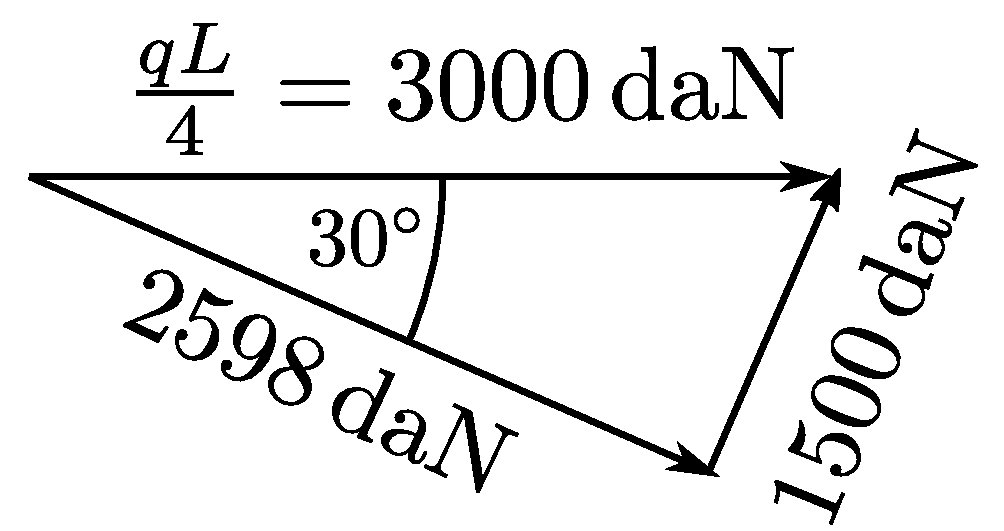
\includegraphics[width=0.45\textwidth]{Immagini/Parte_11/Esercizio11_1_1/esercizio11_1_5.pdf}
\caption{}
\label{Esercizio11-1-5}
\end{figure}
%----------------------------------------------------------------------------------------
Le componenti della forza concentrata in $C$, cioè lo sforzo nel pendolo $\text{CD}$ nelle direzioni dello sforzo normale e del taglio in $C$ sono proprio uguali ai valori di $\Delta N_{C}$ e $\Delta T_{C}$ calcolati, come si vede in figura~\ref{Esercizio11-1-5}. Il fatto che $\Delta N_{C}$ e $\Delta T_{C}$ coincidano, in valore assoluto, con le componenti secondo $n$ e $t$ della forza concentrata in $C$ non è un caso; il perché sarà chiaro in uno dei prssimi paragrafi. Per la sezione $E_s$ consideriamo le forze che seguono, che sono le sole reazioni della cerniera sul primo tronco:
%----------------------------------------------------------------------------------------
\begin{equation*}
\text{Sezione } E_{s} 
\begin{cases}
M_{\textup{E, s}} &=  0 \\
N_{\textup{E, s}} &=  - \frac{3}{4}qL = -\SI{9000}{daN} \\
T_{\textup{E, s}} & = -\frac{qL}{8} = -\SI{1500}{daN}
\end{cases}
\end{equation*}
%----------------------------------------------------------------------------------------
Per la sezione $E_d$ consideriamo le forze che precedono, che sono le sole reazioni della cerniera sul secondo tronco:
%----------------------------------------------------------------------------------------
\begin{equation*}
\text{Sezione } E_{d} 
\begin{cases}
M_{\textup{E, d}} &=  0 \\
N_{\textup{E, d}} &=  - \frac{3}{4}qL = -\SI{9000}{daN} \\
T_{\textup{E, d}} & = -\frac{qL}{8} = -\SI{1500}{daN}
\end{cases}
\end{equation*}
%----------------------------------------------------------------------------------------
Esaminiamo ora la sezione $D_s$, considerando le forze che precedono:
%----------------------------------------------------------------------------------------
\begin{align*}
M_{\textup{D, s}} &= \frac{qL}{8}\cdot \frac{\sqrt{3}}{2}L + \frac{3}{4}qL \cdot \frac{L}{2} - \frac{\sqrt{3}}{2}qL \cdot \frac{\sqrt{3}}{4}L = \frac{\sqrt{3}}{16} qL^{2} = \SI{5196}{daN.m} \\
N_{\textup{D, s}} &= \frac{qL}{8}\cdot \frac{\sqrt{3}}{2} - \frac{\sqrt{3}}{2}qL \cdot \frac{\sqrt{3}}{2} - \frac{3}{4}qL\frac{1}{2} = - \frac{18-\sqrt{3}}{16} qL = - \SI{12201}{daN} \\
T_{\textup{D, s}} &= - \frac{qL}{8} \cdot \frac{1}{2} + \frac{\sqrt{3}}{2}qL\cdot \frac{1}{2} - \frac{3}{4}qL \cdot \frac{\sqrt{3}}{2} = -\frac{1+\sqrt{3}}{16}qL = -\SI{2049}{daN}
\end{align*}
%----------------------------------------------------------------------------------------
Dunque, abbiamo:
%----------------------------------------------------------------------------------------
\begin{equation*}
\text{Sezione } D_{s} 
\begin{cases}
M_{\textup{D, s}} &=  \SI{5196}{daN.m} \\
N_{\textup{D, s}} &=  -\SI{12201}{daN} \\
T_{\textup{D, s}} & = -\SI{2049}{daN}
\end{cases}
\end{equation*}
%----------------------------------------------------------------------------------------
Abbiamo poi la sezione $D_d$, considerando le forze che seguono:
%----------------------------------------------------------------------------------------
\begin{align*}
M_{\textup{D, d}} &= \frac{7}{8}qL\cdot \biggl( 1 - \frac{\sqrt{3}}{2}\biggr)\cdot L - \biggl(1 - \frac{\sqrt{3}}{2} \biggr) \cdot qL \cdot \biggl(1 - \frac{\sqrt{3}}{2}\biggr) \cdot L = \frac{\sqrt{3}}{16} qL^{2} = \SI{5196}{daN.m} \\
N_{\textup{D, d}} &= \frac{7}{8}qL\cdot \frac{\sqrt{3}}{2} + \biggl(1 - \frac{\sqrt{3}}{2}\biggr)\cdot qL\cdot \frac{\sqrt{3}}{2} = - \frac{12-\sqrt{3}}{16} qL = - \SI{7701}{daN} \\
T_{\textup{D, d}} &=  \frac{7}{8}qL\cdot \frac{1}{2} - \biggl(1 - \frac{\sqrt{3}}{2}\biggr)\cdot qL \cdot \frac{1}{2} = \frac{4\cdot \sqrt{3}-1}{16}qL = \SI{4446}{daN}
\end{align*}
%----------------------------------------------------------------------------------------
Pertanto, si ottiene:
%----------------------------------------------------------------------------------------
\begin{equation*}
\text{Sezione } D_{d} 
\begin{cases}
M_{\textup{D, d}} &=  \SI{5196}{daN.m} \\
N_{\textup{D, d}} &=  -\SI{7701}{daN} \\
T_{\textup{D, d}} & = \SI{4446}{daN}
\end{cases}
\end{equation*}
%----------------------------------------------------------------------------------------
Infine, per la sezione $B$ andiamo a considerare l'unica forza che segue:
%----------------------------------------------------------------------------------------
\begin{equation*}
\text{Sezione } B 
\begin{cases}
M_{B} &= 0 \\
N_{B} &= -\frac{7}{8}qL =  -\SI{10500}{daN} \\
T_{B} & = 0
\end{cases}
\end{equation*}
%----------------------------------------------------------------------------------------
%----------------------------------------------------------------------------------------
%----------------------------------------------------------------------------------------
%----------------------------------------------------------------------------------------
%----------------------------------------------------------------------------------------
%----------------------------------------------------------------------------------------
%----------------------------------------------------------------------------------------
%----------------------------------------------------------------------------------------
%----------------------------------------------------------------------------------------
%----------------------------------------------------------------------------------------
%----------------------------------------------------------------------------------------
%----------------------------------------------------------------------------------------
%----------------------------------------------------------------------------------------
%----------------------------------------------------------------------------------------
%----------------------------------------------------------------------------------------
%----------------------------------------------------------------------------------------
%----------------------------------------------------------------------------------------
%----------------------------------------------------------------------------------------